

Avendo definito i principali metodi di navigatione tra ViewController al capitolo~\ref{CH:2} torniamo al problema iniziale:
\textit{Come possiamo rendere dinamica la navigazione?}

A seguito di uno studio approfondito di varie tecniche di navigazione iOS ho scelto di utilizzare il
\textbf{Coordinator Pattern}\cite{coordinatorpattern}.

\section{Il Coordinator Pattern}

Generalmente in iOS l'intera logica di un ViewController viene scritta nel controller stesso, creando spesso
file di grosse dimensioni e disordine generale. Il Coordinator Pattern è nato proprio per rendere 
le applicazioni più scalabili e leggere. 

Ogni ViewController infatti delega tutte le decisioni al suo Coordinator che in base a determinate logiche deciderà
i passi successivi.

Ogni Coordinator può controllare un ViewController o più Coordinator, questo rende le viste
indipendenti tra di loro e rende ogni ViewControler totalmente invisibile agli altri.\\

\begin{minipage}{\linewidth}
    \centering
    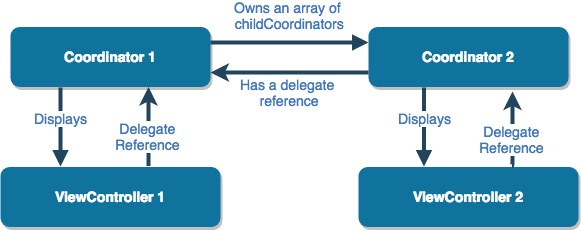
\includegraphics[width=10cm]{coordinator}
    \captionof{figure}{
        Il Coordinator Pattern
    }
    \label{fig:4}
\end{minipage}\\ \\

La resposibilità dei coordinator è infatti la navigazione, come un navigation controller gestisce i sui View Controller, un coordinator gestisce
i suoi figli e questo rende ogni vista o flow di navigazione totalmente indipendente dal resto dell'applicazione.

Per navigare tra i view controller vengono generalmente usate le tipologie di navigazione
descritte nella sezione~\ref{sec:navigation}, tranne le segue, che essendo definete da vista grafica renderebbero
la navigazine statica e fissata su determinati ViewController. \\

Di seguito in figura~\ref{fig:5} presento uno schema dell'utilizzo di due coordinator
per la gestione di una lista di prodotti e il carrello. \\

\begin{minipage}{\linewidth}
    \centering
    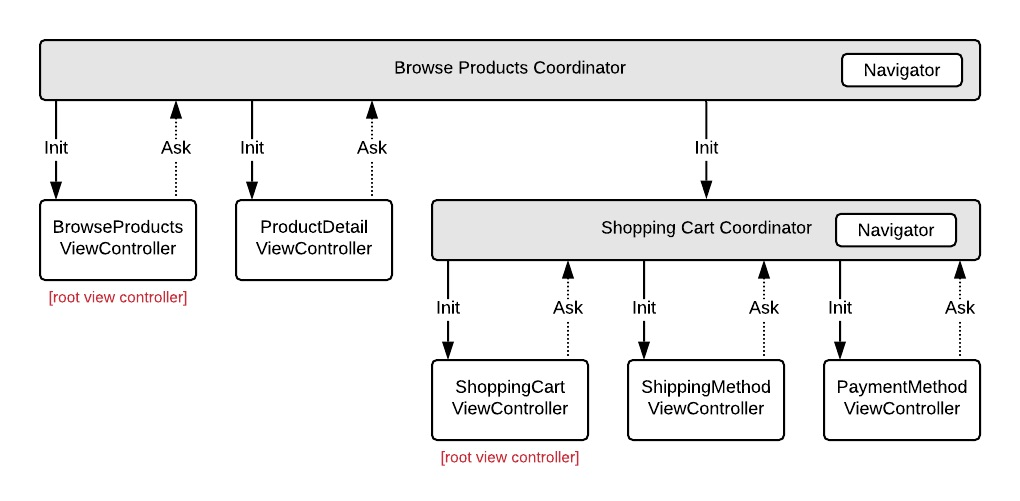
\includegraphics[width=10cm]{coordinator-example}
    \captionof{figure}{
       Esempio di coordinator pattern
    }
    \label{fig:5}
\end{minipage}\\ \\

Come si evince dall'immagine è presente in entrambi i coordinator è presente un oggetto
\textbf{navigator} che sarà in gestore di un UINavigationController